\documentclass[10pt]{article}
\usepackage{fontspec}
\usepackage{polyglossia}
\setdefaultlanguage{ukrainian}
\setotherlanguage{english}
\setmainfont{Liberation Sans}
\setmonofont{DejaVu Sans Mono}[Scale=0.85]
\usepackage[papersize={9cm,16cm},margin=0.55cm,top=0.5cm,bottom=0.6cm]{geometry}
\usepackage{amsmath,amssymb}
\usepackage{graphicx}
\usepackage{booktabs}
\usepackage{xcolor}
\usepackage{tikz}
\usetikzlibrary{positioning,arrows.meta}
\usepackage{enumitem}
\setlist{leftmargin=1.1em,itemsep=2pt,topsep=2pt}
\pagestyle{empty}
\setlength{\parindent}{0pt}
\definecolor{acc}{HTML}{1D6F72}
\definecolor{bad}{HTML}{C0533A}
\newcommand{\slidetitle}[1]{{\color{acc}\Large\bfseries #1}\par\vspace{1mm}{\color{acc}\rule{\linewidth}{1pt}}\par\vspace{2.5mm}}
\newcommand{\num}[2]{\hfill\textcolor{gray}{\footnotesize #1/#2}}
\newcommand{\code}[1]{\texttt{#1}}
\sloppy

\begin{document}

% 1 -------------------------------------------------------------------
\vspace*{1.2cm}
{\color{acc}\small Комп'ютерний практикум № 4}\par\vspace{3mm}
{\Huge\bfseries DQN\\[1mm] в Acrobot-v1}\par\vspace{4mm}
{\large Як гіперпараметри впливають на навчання і поведінку агента}\par\vspace{8mm}
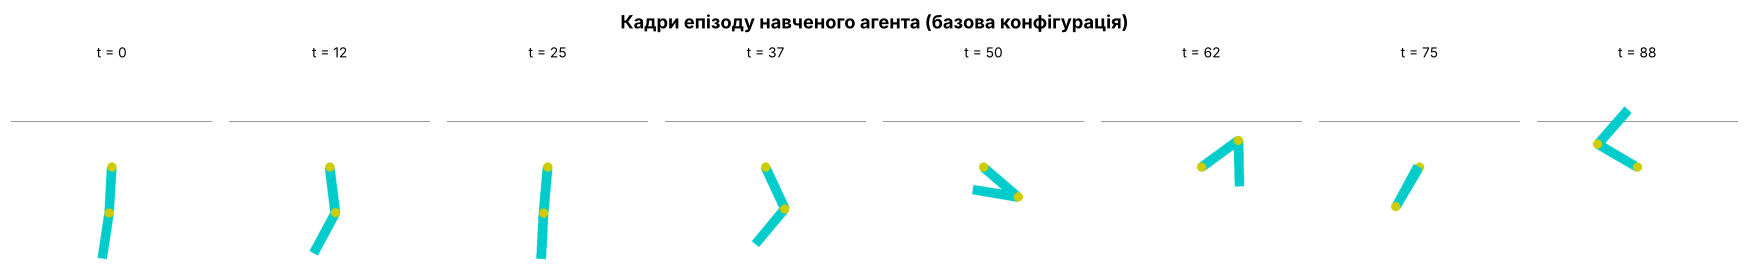
\includegraphics[width=\linewidth]{../fig_frames.png}\par\vspace{8mm}
\begin{tabular}{@{}ll@{}}
Метод: & Deep Q-Network\\
Реалізація: & Stable-Baselines3\\
Базова конфіг.: & RL Baselines3 Zoo\\
Експерименти: & 9 конфіг. $\times$ 3 seed\\
\end{tabular}
\vfill
{\small Основи глибокого навчання з підкріпленням, КПІ 2026}
\newpage

% 2 -------------------------------------------------------------------
\slidetitle{Задача}
\textbf{Acrobot} — дволанковий маятник із приводом лише в середньому шарнірі. Треба розгойдати його, щоб кінець нижньої ланки піднявся вище лінії.\par\vspace{3mm}
\begin{tabular}{@{}p{2.2cm}p{5.2cm}@{}}\toprule
Стан & 6 чисел: cos/sin двох кутів, дві кутові швидкості \\[1mm]
Дії & 3 дискретні: момент $-1$, $0$, $+1$ \\[1mm]
Винагорода & $-1$ за кожен крок до цілі \\[1mm]
Кінець & ціль досягнута (terminated) або 500 кроків (truncated) \\[1mm]
Якість & середній дохід; $-500$ = провал, поріг «розв'язано» $-100$ \\ \bottomrule
\end{tabular}\par\vspace{5mm}
\textbf{Чому складно:} винагорода розріджена — випадкова політика ніколи не досягає цілі (усі 20 спроб: $-500$). Одним рухом ціль недосяжна, потрібно накопичувати енергію серією узгоджених дій.
\vfill\num{2}{8}
\newpage

% 3 -------------------------------------------------------------------
\slidetitle{Метод: DQN}
Q-learning, де таблицю замінено нейромережею $Q_\theta(s,a)$.\par\vspace{2mm}
\textbf{Value-based · model-free · off-policy}\par\vspace{3mm}
\textbf{Ціль і втрата}
\[
y=r+\gamma(1-d)\max_{a'}Q_{\theta^-}(s',a')
\]
\[
L(\theta)=\mathrm{Huber}\bigl(Q_\theta(s,a)-y\bigr)\ \to\ \text{Adam}
\]
\textbf{Два стабілізатори}
\begin{itemize}
\item \textbf{Буфер відтворення} (50k переходів): випадкові батчі по 128 руйнують кореляції, досвід використовується повторно.
\item \textbf{Цільова мережа} $Q_{\theta^-}$: копія ваг кожні 250 кроків — ціль «заморожена».
\end{itemize}\vspace{2mm}
\textbf{Дослідження:} $\varepsilon$-жадібно, $\varepsilon$: $1\to0.1$ за перші 12\,\% кроків. Оцінювання — жадібно ($\varepsilon=0$).
\vfill\num{3}{8}
\newpage

% 4 -------------------------------------------------------------------
\slidetitle{Архітектура}
\begin{center}
\begin{tikzpicture}[node distance=0.5cm, >=Stealth, every node/.style={font=\small},
  box/.style={draw, rounded corners, minimum width=4.6cm, minimum height=0.85cm, align=center, fill=#1}, box/.default=blue!8]
\node[box=gray!12] (in) {вхід: стан $s\in\mathbb R^6$};
\node[box, below=of in] (h1) {Linear 6$\to$256 + ReLU};
\node[box, below=of h1] (h2) {Linear 256$\to$256 + ReLU};
\node[box=orange!18, below=of h2] (out) {Linear 256$\to$3: $Q(s,-1),Q(s,0),Q(s,+1)$};
\node[box=gray!12, below=of out] (act) {дія $=\arg\max_a Q(s,a)$};
\draw[->] (in)--(h1); \draw[->] (h1)--(h2); \draw[->] (h2)--(out); \draw[->] (out)--(act);
\end{tikzpicture}
\end{center}
Дві однакові мережі: \textbf{Q-net} (навчається) і \textbf{target} (лише для цілі $y$).\par\vspace{3mm}
\begin{tabular}{@{}lr@{}}\toprule
Досліджені варіанти & параметрів\\ \midrule
{[256, 256]} (базова) & 68\,355\\
{[64, 64]} & 4\,803\\
{[16]} & 163\\ \bottomrule
\end{tabular}
\vfill\num{4}{8}
\newpage

% 5 -------------------------------------------------------------------
\slidetitle{План експериментів}
Один змінений гіперпараметр відносно базової конфігурації; 3 seed; 60\,000 кроків; оцінювання — 50 жадібних епізодів.\par\vspace{3mm}
\begin{tabular}{@{}p{2.4cm}p{5.0cm}@{}}\toprule
\textbf{Крок навчання} & $10^{-4}$, \textbf{6.3e-4}, $3\cdot10^{-3}$\\[1mm]
\textbf{Цільова мережа} & кожні 10, \textbf{250}, 2000 кроків\\[1mm]
\textbf{Архітектура} & [16], [64,64], \textbf{[256,256]}\\[1mm]
\textbf{Дослідження} & \textbf{(0.12, 0.1)}; частка 0.5; $\varepsilon_{\text{final}}=0.01$\\ \bottomrule
\end{tabular}\par\vspace{4mm}
\textbf{Чому саме ці?} По одному параметру з кожного компонента DQN: оптимізація, стабілізація цілі, апроксиматор, дослідження. Значення — у 5–10 разів по обидва боки від базового, щоб ефект перевищував шум між seed.
\vfill\num{5}{8}
\newpage

% 6 -------------------------------------------------------------------
\slidetitle{Результати}
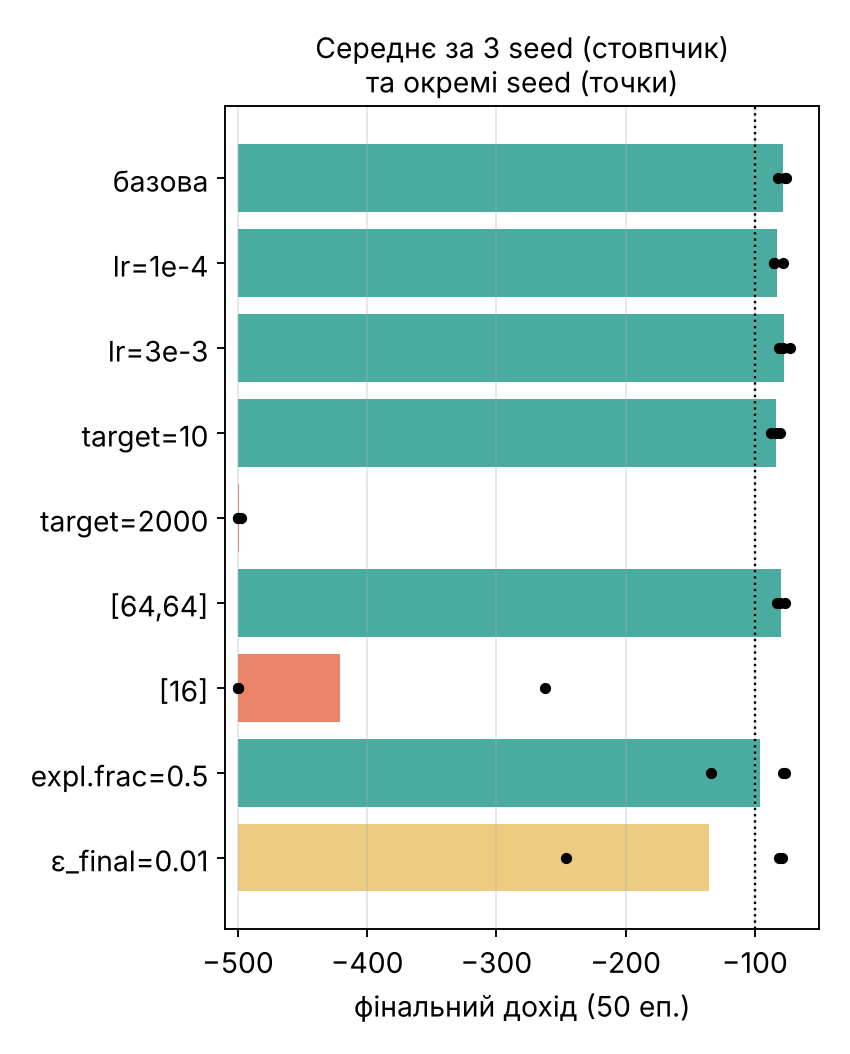
\includegraphics[width=\linewidth]{../fig_slide_bars.png}\par\vspace{2mm}
\begin{itemize}
\item Базова: $\mathbf{-78.0\pm2.7}$, 100\,\% успіхів (RL Zoo, $10^5$ кроків: $-72.1$).
\item \code{lr} у межах $10^{-4}$–$3\cdot10^{-3}$: усе навчається, різниця — у швидкості та коливаннях.
\item \textcolor{bad}{\textbf{target = 2000}} і \textcolor{bad}{\textbf{[16]}} — провал.
\item {[64,64]} рівноцінна базовій і вдвічі швидша.
\end{itemize}
\vfill\num{6}{8}
\newpage

% 7 -------------------------------------------------------------------
\slidetitle{Чому агент провалюється}
\begin{center}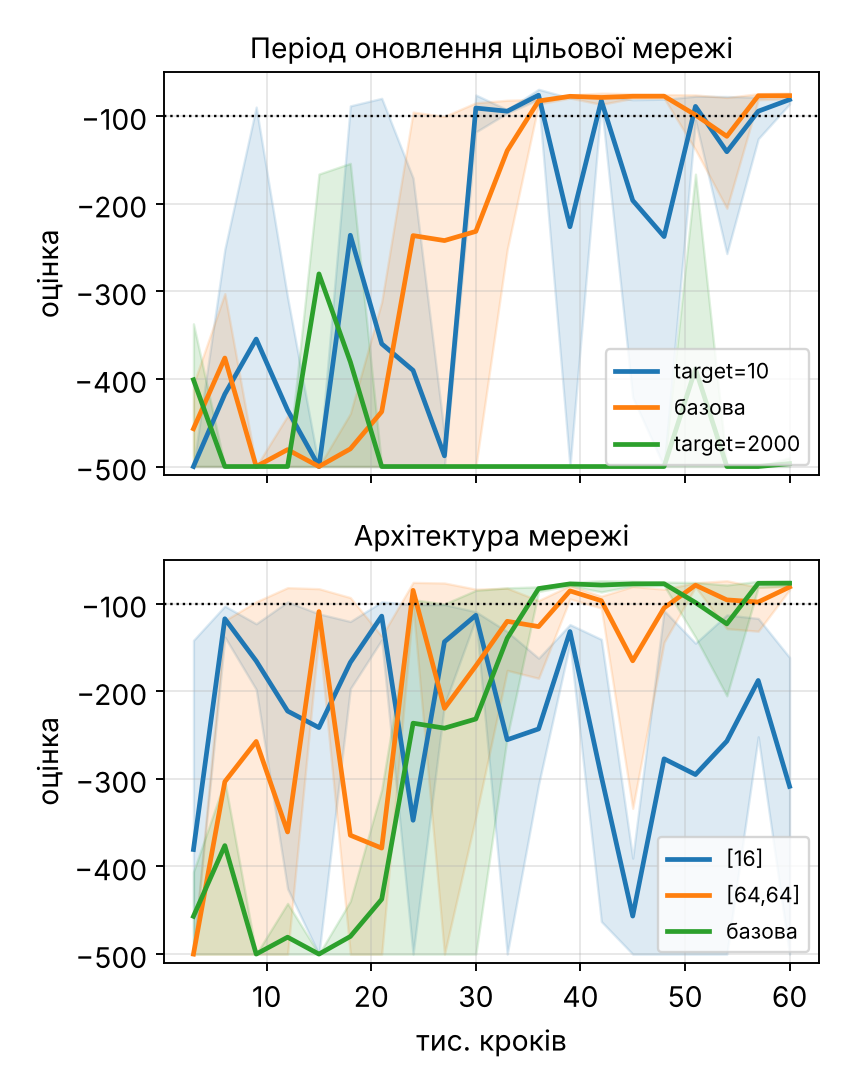
\includegraphics[height=7.6cm]{../fig_slide_curves.png}\end{center}\vspace{-2mm}\par\vspace{2mm}
У невдалих запусках жадібна політика \textbf{вироджується в одну дію} (91–100\,\% кроків — той самий момент): маятник не розгойдується.\par\vspace{1.5mm}
\textbf{Причина — малий action gap:} різниця Q дій $\approx0.6$ при $|Q|\approx30$ (2\,\%). Мала мережа чи застаріла ціль цю різницю «губить». $\varepsilon$-шум у навчанні маскує дефект.
\vfill\num{7}{8}
\newpage

% 8 -------------------------------------------------------------------
\slidetitle{Висновки}
\begin{enumerate}
\item DQN зі SB3 стабільно розв'язує Acrobot за 60k кроків і знаходить фізично осмислену стратегію «розгойдування» моментами $\pm1$.
\item \textbf{Цільова мережа} — найчутливіший параметр: 10 — швидко, але нестабільно; 2000 — цінності не встигають поширитися.
\item \textbf{Крок навчання} впливає на швидкість, не на результат (Adam + Huber + clip).
\item \textbf{Мережа} [64,64] достатня; [16] — ні.
\item \textbf{Дослідження:} базовий розклад найнадійніший.
\item Якість DQN треба мірити \textbf{жадібно, на багатьох епізодах і seed}: навчальні криві можуть вводити в оману.
\end{enumerate}\vspace{2mm}
{\small\textbf{Обмеження:} 3 seed, 60k кроків замість 100k, одне середовище, один параметр за раз.}
\vfill\num{8}{8}

\end{document}
